\documentclass[12pt]{article} % use larger type; default would be 10pt

\usepackage{tikz}
\usepackage{pgfplots}
\usetikzlibrary{calc}
\usetikzlibrary{arrows.meta}
\usetikzlibrary{patterns}
        \newcommand\degree[0]{^{\circ}}
\usetikzlibrary{shapes.misc}

\title{Play with TikZ}
\author{Just Us}
%\date{} % Activate to display a given date or no date (if empty),
         % otherwise the current date is printed 

\begin{document}
\maketitle

\section{Chap 4 Trigonometric Functions}

\subsection{Review Problems}

hp4-sum-7 grid
\newline
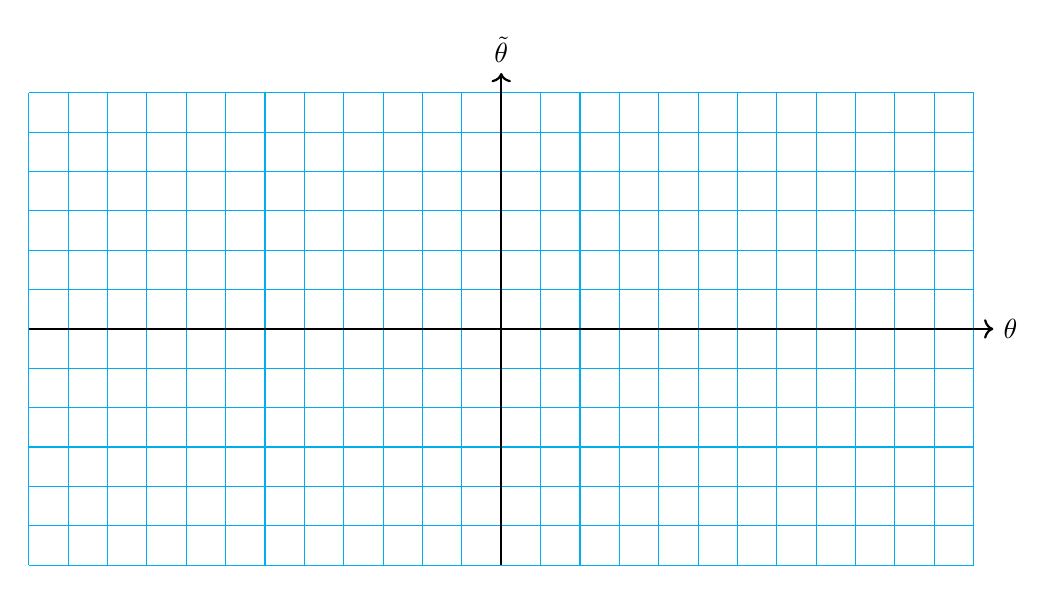
\begin{tikzpicture} [scale=.5]
\draw[cyan] (-12, -6) grid (12,6);
\draw[black, thick, ->] (-12,0)--(12.5,0) node[right]{$\theta$};
\draw[black, thick, ->] (0,-6)--(0,6.5) node[above]{$\tilde{\theta}$};

\end{tikzpicture}
\newline

hp4-sum-7ans referance angle vs angle

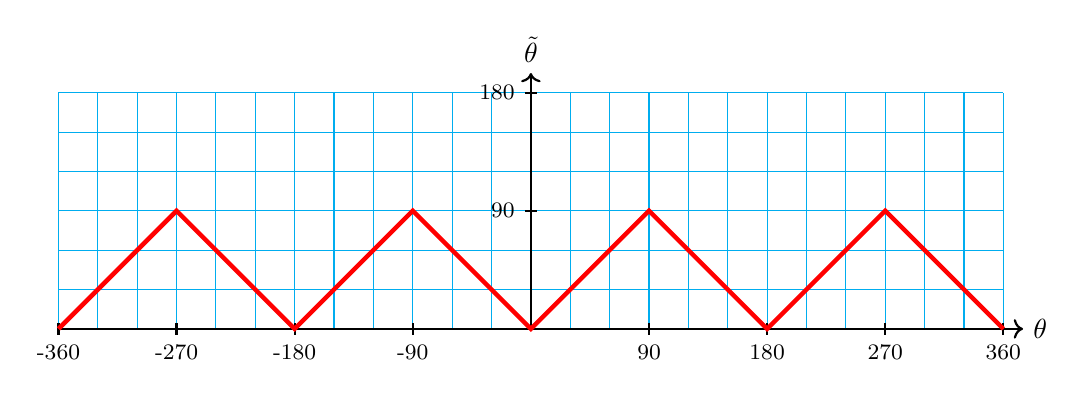
\begin{tikzpicture} [scale=.5]
\draw[cyan] (-12, 0) grid (12,6);
\draw[black, thick, ->] (-12,0)--(12.5,0) node[right]{$\theta$};
\draw[black, thick, ->] (0,0)--(0,6.5) node[above]{$\tilde{\theta}$};

\foreach \x [evaluate=\x as \xi using int(30*\x)] in {-12, -9, -6, -3, 3, 6, 9, 12}
 \draw[black, thick] (\x, 0.15)--++(0, -.3) node[below]{\footnotesize \xi};
\foreach \y [evaluate=\y as \yi using int(30*\y)] in {3, 6}
 \draw[black, thick] (0.15,\y)--++(-.3,0) node[left]{\footnotesize \yi};
 
\draw[red, ultra thick] (-12, 0) --++(3,3)--++(3,-3) --++(3,3) --++(3,-3) --++(3,3) --++(3,-3) --++(3,3) --++(3,-3);

\end{tikzpicture}
\newline

hp4-sum-35ans sinusoidal graph

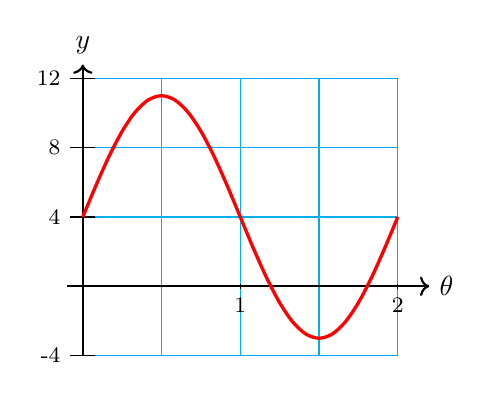
\begin{tikzpicture} [xscale=2, yscale=.22]
\draw[cyan, xstep=.5, ystep=4] (0, -4) grid (2,12);
\draw[black, thick, ->] (-0.1,0)--(2.2,0) node[right]{$\theta$};
\draw[black, thick, ->] (0,-4)--(0,12.8) node[above]{$y$};

\foreach \x in {1,2}
 \draw[black] (\x, 0.15)--++(0, -.3) node[below]{\footnotesize \x};
\foreach \y  in {-4, 4, 8, 12}
 \draw[black] (0.08,\y)--++(-.16,0) node[left]{\footnotesize \y};
 
\draw[domain=0:2,smooth,variable=\x,red,very thick] plot ({\x},{4+ 7*sin(180*\x)});

\end{tikzpicture}
\newline

hp4-sum-37ans sinusoidal graph

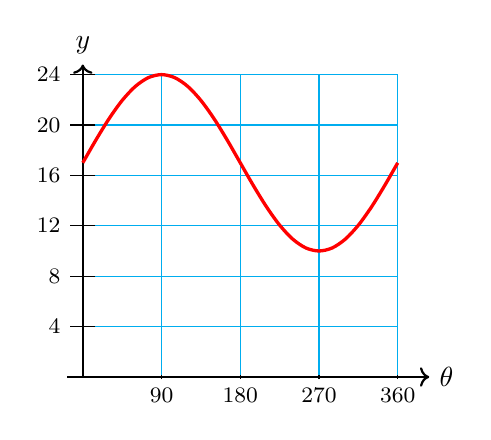
\begin{tikzpicture} [xscale=2, yscale=.16]
\draw[cyan, xstep=.5, ystep=4] (0, 0) grid (2,24);
\draw[black, thick, ->] (-0.1,0)--(2.2,0) node[right]{$\theta$};
\draw[black, thick, ->] (0,0)--(0,24.8) node[above]{$y$};

\foreach \x  [evaluate =\x as \xi using int(180*\x)] in {.5, 1, 1.5, 2}
 \draw[black] (\x, 0.15)--++(0, -.3) node[below]{\footnotesize \xi};
\foreach \y  in {4, 8, ..., 24}
 \draw[black] (0.08,\y)--++(-.16,0) node[left]{\footnotesize \y};
 
\draw[domain=0:2,smooth,variable=\x,red,very thick] plot ({\x},{17+ 7*sin(180*\x)});

\end{tikzpicture}
\newline

hp4-sum-43 sinusoidal graph

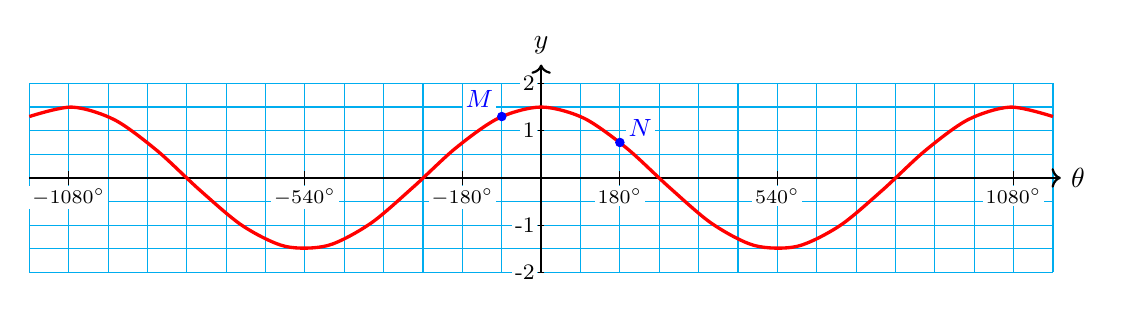
\begin{tikzpicture} [xscale=.5, yscale=.6]
\draw[cyan, ystep=.5] (-13,-2) grid (13,2);
\draw[black, thick, ->] (-13,0)--(13.2,0) node[right]{$\theta$};
\draw[black, thick, ->] (0,-2)--(0,2.4) node[above]{$y$};

\foreach \x  [evaluate =\x as \xi using int(90*\x)] in {-12, -6, -2, 2, 6, 12}
 \draw[black] (\x, 0.15)--++(0, -.3) node[below, fill=white, inner sep=1pt]{\scriptsize $\xi\degree$};
\foreach \y  in {-2, -1, 1, 2}
 \draw[black] (0.08,\y)--++(-.16,0) node[left, fill=white, inner sep=1pt]{\footnotesize \y};
 
\draw[domain=-13:13,smooth,variable=\x,red,very thick] plot ({\x},{1.5*cos(90*\x/3)});

\coordinate (M) at ($ 1.5*cos(30)*(0,1) + (-1,0)$);
\filldraw[blue] (M) ellipse (3pt and 2.5pt) node[anchor=south east, xshift=-2, yshift=2, fill=white, inner sep=1pt] {\small $M$};

\coordinate (N) at ($ 1.5*cos(60)*(0,1) + (2,0)$);

\filldraw[blue] (N) ellipse (3pt and 2.5pt) node[anchor=south west, xshift=2, yshift=1, fill=white, inner sep=1pt] {\small $N$};

\end{tikzpicture}
\newline

hp4-sum-44 sinusoidal graph

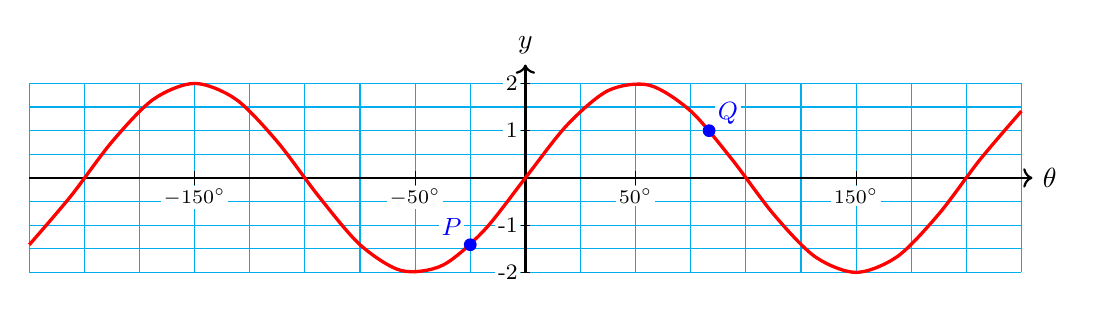
\begin{tikzpicture} [xscale=.7, yscale=.6]
\draw[cyan, ystep=.5] (-9,-2) grid (9,2);
\draw[black, thick, ->] (-9,0)--(9.2,0) node[right]{$\theta$};
\draw[black, thick, ->] (0,-2)--(0,2.4) node[above]{$y$};

\foreach \x  [evaluate =\x as \xi using int(25*\x)] in {-6, -2, 2, 6}
 \draw[black] (\x, 0.15)--++(0, -.3) node[below, fill=white, inner sep=1pt]{\scriptsize $\xi\degree$};
\foreach \y  in {-2, -1, 1, 2}
 \draw[black] (0.08,\y)--++(-.16,0) node[left, fill=white, inner sep=1pt]{\footnotesize \y};
 
\draw[domain=-9:9,smooth,variable=\x,red,very thick] plot ({\x},{2*sin(25*\x *9/5)});

\coordinate (P) at ($ 2*sin(-45)*(0,1) + (-1,0)$);
\filldraw[blue] (P) ellipse (3pt and 3.5pt) node[anchor=south east, xshift=-2, yshift=2, fill=white, inner sep=1pt] {\small $P$};

\coordinate (Q) at ($ 10/3*(1,0) + (0,1) $);

\filldraw[blue] (Q) ellipse (3pt and 3.5pt) node[anchor=south west, xshift=2, yshift=1, fill=white, inner sep=1pt] {\small $Q$};

\end{tikzpicture}
\newline

hp4-sum-45 sinusoidal graph

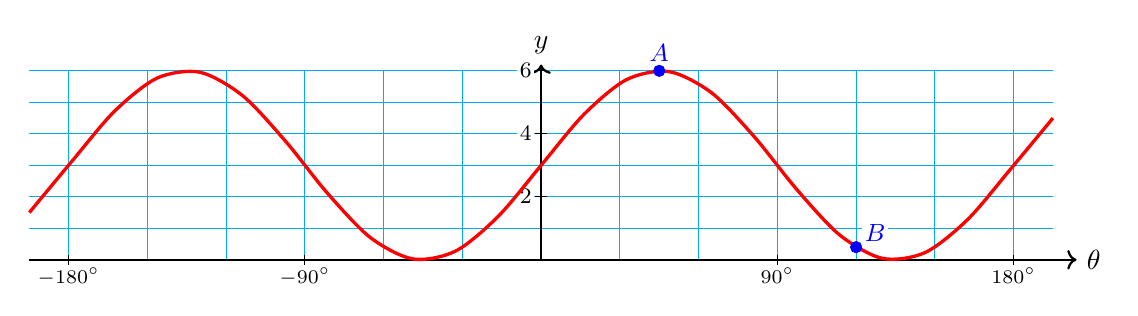
\begin{tikzpicture} [xscale=1, yscale=.4]
\draw[cyan] (-6.5,0) grid (6.5,6);
\draw[black, thick, ->] (-6.5,0)--(6.8,0) node[right]{$\theta$};
\draw[black, thick, ->] (0,0)--(0,6.2) node[above]{$y$};

\foreach \x  [evaluate =\x as \xi using int(30*\x)] in {-6, -3, 3, 6}
 \draw[black] (\x, 0.15)--++(0, -.3) node[below, fill=white, inner sep=1pt]{\scriptsize $\xi\degree$};
\foreach \y  in {2, 4, 6}
 \draw[black] (0.08,\y)--++(-.16,0) node[left, fill=white, inner sep=1pt]{\footnotesize \y};
 
\draw[domain=-6.5:6.5,smooth,variable=\x,red,very thick] plot ({\x},{3+3*sin(30*\x *2)});

\coordinate (A) at (1.5,6);
\filldraw[blue] (A) ellipse (2pt and 5pt) node[anchor=south ,  yshift=2, fill=white, inner sep=1pt] {\small $A$};

\coordinate (B) at ($ 3*sin(240)*(0,1) + (4,3) $);

\filldraw[blue] (B) ellipse (2pt and 5pt) node[anchor=south west, xshift=2, yshift=1, fill=white, inner sep=1pt] {\small $B$};

\end{tikzpicture}
\newline

hp4-sum-46 sinusoidal graph

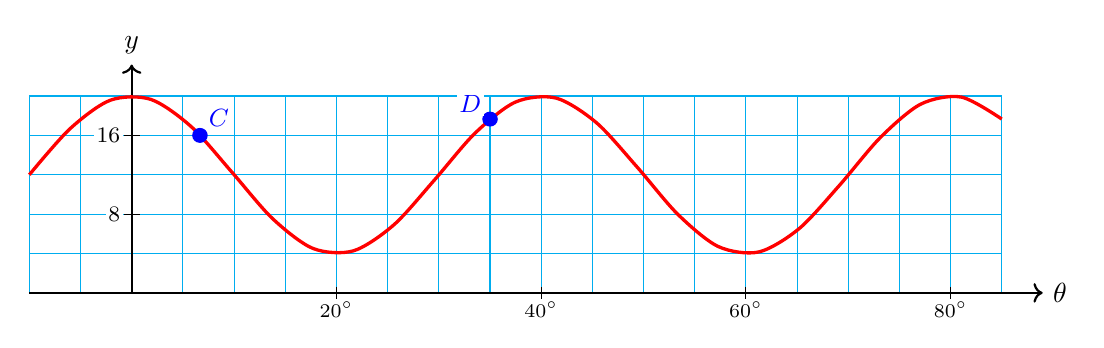
\begin{tikzpicture} [xscale=1.3, yscale=.5]
\draw[cyan, xstep=.5] (-1,0) grid (8.5,5);
\draw[black, thick, ->] (-1,0)--(8.9,0) node[right]{$\theta$};
\draw[black, thick, ->] (0,0)--(0,5.8) node[above]{$y$};

\foreach \x  [evaluate =\x as \xi using int(10*\x)] in {2, 4, 6, 8}
 \draw[black] (\x, 0.15)--++(0, -.3) node[below, fill=white, inner sep=1pt]{\scriptsize $\xi\degree$};
\foreach \y [evaluate=\y as \yi using int(4*\y)] in {2, 4}
 \draw[black] (0.08,\y)--++(-.16,0) node[left, fill=white, inner sep=1pt]{\footnotesize \yi};
 
\draw[domain=-1:8.5,smooth,variable=\x,red,very thick] plot ({\x},{3+2*cos(10*\x *9)});

\coordinate (C) at (2/3,4);
\filldraw[blue] (C) ellipse (2pt and 5pt) node[anchor=south west, xshift=2, yshift=2, fill=white, inner sep=1pt] {\small $C$};

\coordinate (D) at ($ 2*cos(315)*(0,1) + (3.5,3) $);

\filldraw[blue] (D) ellipse (2pt and 5pt) node[anchor=south east, xshift=-2, yshift=1, fill=white, inner sep=1pt] {\small $D$};

\end{tikzpicture}
\newline

hp4-sum-47ans periodic doses of drug

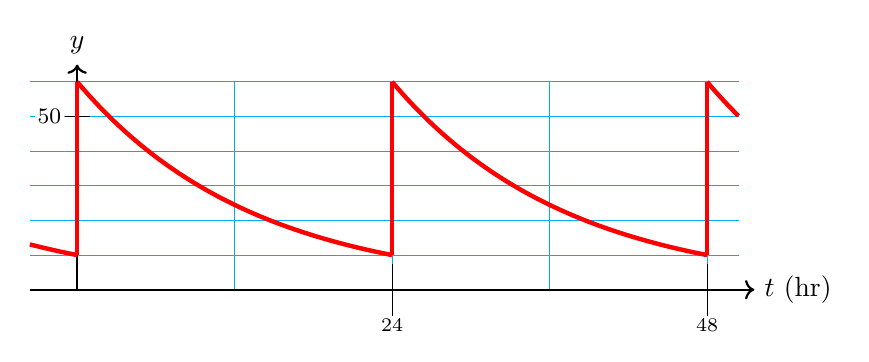
\begin{tikzpicture} [xscale=2, yscale=2.2]
\draw[cyan, ystep=.2] (-.3,0) grid (4.2,1.2);
\draw[black, thick, ->] (-.3,0)--(4.3,0) node[right]{$t$ (hr)};
\draw[black, thick, ->] (0,0)--(0,1.3) node[above]{$y$};

\foreach \x  [evaluate =\x as \xi using int(12*\x)] in {2,4}
 \draw[black] (\x, 0.15)--++(0, -.3) node[below, fill=white, inner sep=1pt]{\scriptsize \xi};
\foreach \y [evaluate=\y as \yi using int(50*\y)] in {1}
 \draw[black] (0.08,\y)--++(-.16,0) node[left, fill=white, inner sep=1pt]{\footnotesize \yi};
 
\draw[domain=-.3:0,smooth,variable=\x,red,ultra thick] plot ({\x},{ 1.2/6^((\x+2) /2))});
\draw[red,ultra thick] (0,1.2)--++(0,-1);

\draw[domain=0:2,smooth,variable=\x,red,ultra thick] plot ({\x},{ 1.2/6^(\x /2))});
\draw[red,ultra thick] (2,1.2)--++(0,-1);

\draw[domain=2:4,smooth,variable=\x,red,ultra thick] plot ({\x},{ 1.2/6^((\x-2) /2))});
\draw[red,ultra thick] (4,1.2)--++(0,-1);

\draw[domain=4:4.2,smooth,variable=\x,red,ultra thick] plot ({\x},{ 1.2/6^((\x-4) /2))});


\end{tikzpicture}
\newline

hp4-sum-49ans carousel

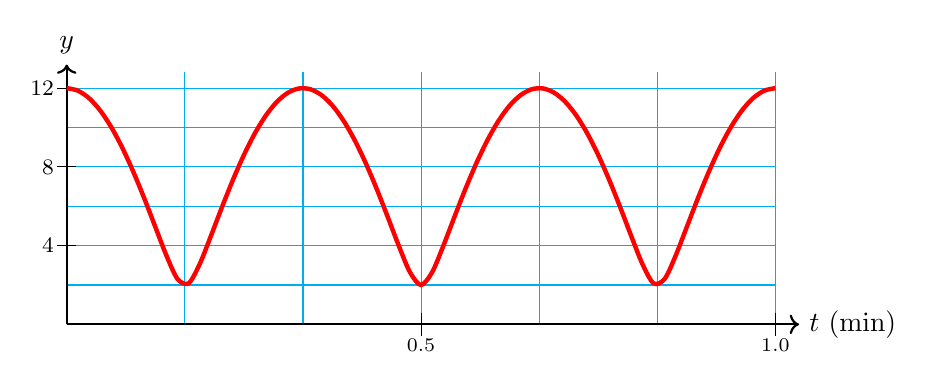
\begin{tikzpicture} [xscale=1.5]
\draw[cyan, ystep=.5] (0,0) grid (6,3.2);
\draw[black, thick, ->] (0,0)--(6.2,0) node[right]{$t$ (min)};
\draw[black, thick, ->] (0,0)--(0,3.3) node[above]{$y$};

\foreach \x  [evaluate =\x as \xi using ( \x /6 )] in {3,6}
 \draw[black] (\x, 0.15)--++(0, -.3) node[below, fill=white, inner sep=1pt]{\scriptsize \xi};
\foreach \y [evaluate=\y as \yi using int(4*\y)] in {1, 2, 3}
 \draw[black] (0.08,\y)--++(-.16,0) node[left, fill=white, inner sep=1pt]{\footnotesize \yi};
 
\draw[samples=65,domain=-0:6,smooth,variable=\x,red,ultra thick] plot ({\x},{ sqrt( (1.25*cos(180*\x) + 1.75)^2 + (1.25*sin(180*\x))^2   ) });

\end{tikzpicture}
\newline

hp4-sum-51ans cosine graph

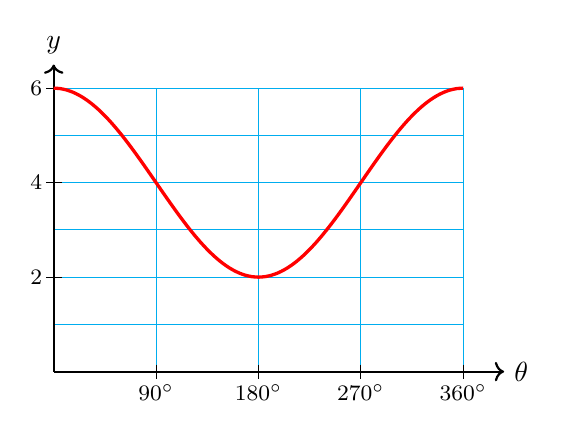
\begin{tikzpicture} [xscale=1.3, yscale=.6]
\draw[cyan] (0,0) grid (4,6);
\draw[black, thick, ->] (0,0)--(4.4,0) node[right]{$\theta$};
\draw[black, thick, ->] (0,0)--(0,6.5) node[above]{$y$};

\foreach \x  [evaluate =\x as \xi using int( \x * 90 )] in {1, 2, 3, 4}
 \draw[black] (\x, 0.15)--++(0, -.3) node[below, fill=white, inner sep=1pt, yshift=-1]{\footnotesize $\xi\degree$};
\foreach \y [evaluate=\y as \yi using int(1*\y)] in {2, 4, 6}
 \draw[black] (0.08,\y)--++(-.16,0) node[left, fill=white, inner sep=1pt]{\footnotesize \yi};
 
\draw[samples=65,domain=-0:4,smooth,variable=\x,red, very thick] plot ({\x},{ 4 + 2*cos(90*\x) ) });

\end{tikzpicture}
\newline

hp4-sum-51ans sine graph

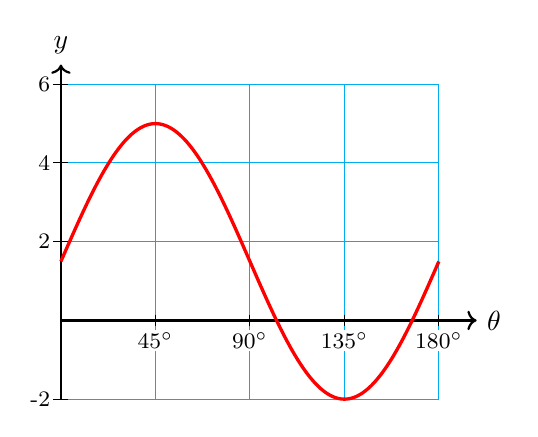
\begin{tikzpicture} [xscale=1.2, yscale=.5]
\draw[cyan, ystep=2] (0,-2) grid (4,6);
\draw[black, thick, ->] (0,0)--(4.4,0) node[right]{$\theta$};
\draw[black, thick, ->] (0,-2)--(0,6.5) node[above]{$y$};

\foreach \x  [evaluate =\x as \xi using int( \x * 45 )] in {1, 2, 3, 4}
 \draw[black] (\x, 0.15)--++(0, -.3) node[below, fill=white, inner sep=1pt, yshift=-1]{\footnotesize $\xi\degree$};
\foreach \y [evaluate=\y as \yi using int(1*\y)] in {-2, 2, 4, 6}
 \draw[black] (0.08,\y)--++(-.16,0) node[left, fill=white, inner sep=1pt]{\footnotesize \yi};
 
\draw[samples=65,domain=-0:4,smooth,variable=\x,red, very thick] plot ({\x},{ 1.5 + 3.5*sin(90*\x) ) });

\end{tikzpicture}
\newline

hp4-sum-63ans tan and cosine graphs

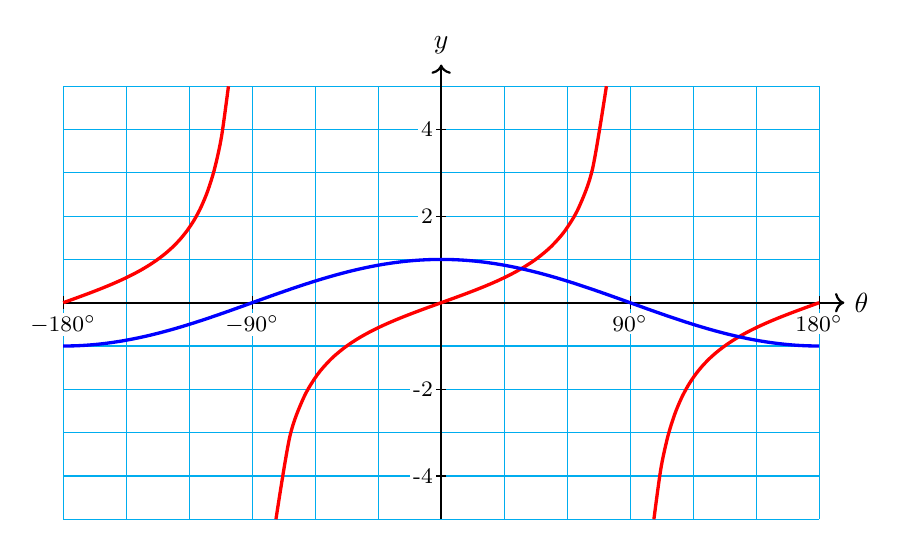
\begin{tikzpicture} [xscale=.8, yscale=.55]
\draw[cyan ] (-6,-5) grid (6,5);
\draw[black, thick, ->] (-6,0)--(6.4,0) node[right]{$\theta$};
\draw[black, thick, ->] (0,-5)--(0,5.5) node[above]{$y$};

\foreach \x  [evaluate =\x as \xi using int( \x * 30 )] in {-6, -3, 3, 6}
 \draw[black] (\x, 0.15)--++(0, -.3) node[below, fill=white, inner sep=1pt, yshift=-1]{\footnotesize $\xi\degree$};
\foreach \y [evaluate=\y as \yi using int(1*\y)] in {-4, -2, 2, 4}
 \draw[black] (0.08,\y)--++(-.16,0) node[left, fill=white, inner sep=1pt]{\footnotesize \yi};

\draw[domain={-6:atan(5)/30 - 6},smooth,variable=\x,red, very thick] plot ({\x},{ tan(30*\x) ) });
\draw[domain={atan(-5)/30:atan(5)/30},smooth,variable=\x,red, very thick] plot ({\x},{ tan(30*\x) ) });
\draw[domain={atan(-5)/30+6:6},smooth,variable=\x,red, very thick] plot ({\x},{ tan(30*\x) ) });

\draw[samples=65,domain=-6:6,smooth,variable=\x,blue, very thick] plot ({\x},{ cos(30*\x) ) });

\end{tikzpicture}
\newline






\section {Stuff for later}




sine graph
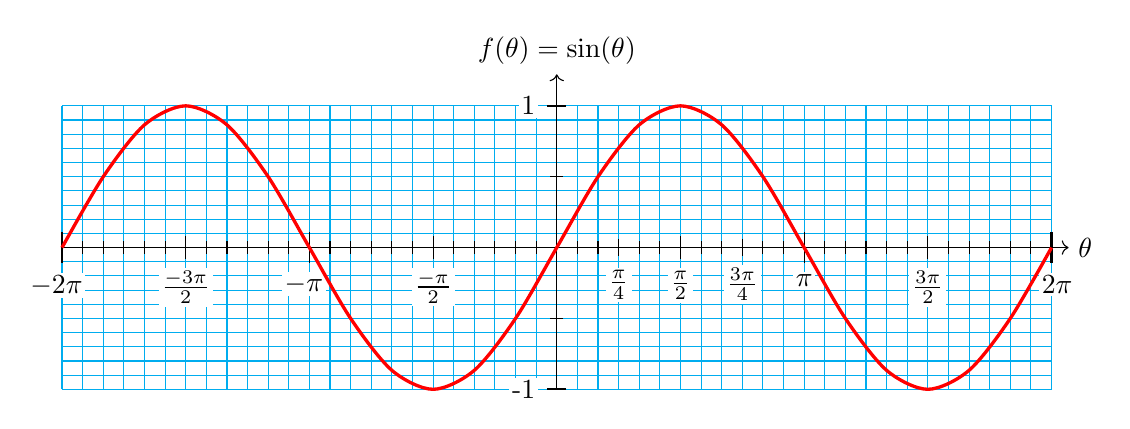
\begin{tikzpicture}

\draw[cyan,xstep=pi/12,ystep=0.18]
(-2*pi,-1.8) grid (2*pi,1.8);

\draw[->] (-6.3,0) -- (6.5,0) node[right] {$\theta$};
\draw[->] (0,-1.8) -- (0,2.2) node[above] {$f(\theta)=\sin(\theta)$};

\foreach \x in {-24,-23,...,24}
\draw[black] ($ pi*\x /12*(1,0) +(0,.08) $) --++(0,-.16);
\foreach \y in {-0.9, 0.9}
\draw[black] (.08,\y ) --++(-.16,0);
\foreach \y in {-1,1}
\draw[black, thick] (.12,1.8*\y ) --++(-.24,0) node[anchor=east, xshift=-3, fill=white, inner sep=1pt] {\y};

\draw[black, thick] (-2*pi,.2) --++(0,-.4) node[anchor=north, xshift=-2,yshift=-3, fill=white, inner sep=1pt] {$-2\pi$};
\draw[black, thick] (2*pi,.2) --++(0,-.4) node[anchor=north, xshift=2,yshift=-3, fill=white, inner sep=1pt] {$2\pi$};

\draw[black] (pi,.2) --++(0,-.4) node[anchor=north, yshift=-3, fill=white, inner sep=1pt] {$\pi$};

\draw[black] (pi,.2) --++(0,-.4) node[anchor=north, yshift=-3, fill=white, inner sep=1pt] {$\pi$};
\draw[black] (-pi,.2) --++(0,-.4) node[anchor=north, xshift=-2,yshift=-3, fill=white, inner sep=1pt] {$-\pi$};
\draw[black] (-pi/2,.15) --++(0,-.3) node[anchor=north, yshift=-3, fill=white, inner sep=1pt] {$\frac{-\pi}{2}$};
\draw[black] (pi/2,.15) --++(0,-.3) node[anchor=north, yshift=-3, fill=white, inner sep=1pt] {$\frac{\pi}{2}$};
\draw[black] (3*pi/2,.15) --++(0,-.3) node[anchor=north, yshift=-3, fill=white, inner sep=1pt] {$\frac{3\pi}{2}$};
\draw[black] (-3*pi/2,.15) --++(0,-.3) node[anchor=north, yshift=-3, fill=white, inner sep=1pt] {$\frac{-3\pi}{2}$};

\draw[black] (pi/4,.11) --++(0,-.22) node[anchor=north, yshift=-4, fill=white, inner sep=1pt] {$\frac{\pi}{4}$};

\draw[black] (3*pi/4,.11) --++(0,-.22) node[anchor=north, yshift=-3, fill=white, inner sep=1pt] {$\frac{3\pi}{4}$};

\draw[domain=-2*pi:2*pi,smooth,variable=\x,red,very thick] plot ({\x},{1.8*sin(deg(\x))});

\end{tikzpicture}
\newline


cosine graph
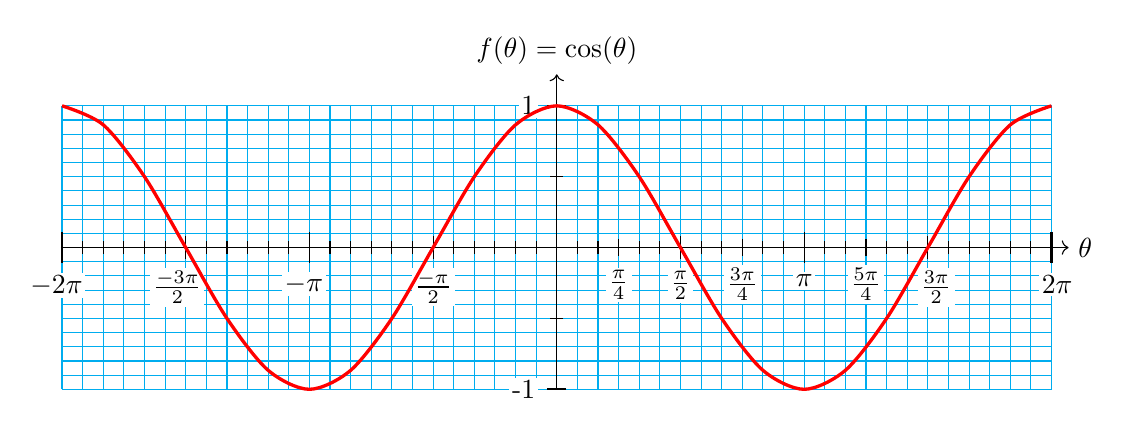
\begin{tikzpicture} 

\draw[cyan,xstep=pi/12,ystep=0.18]
(-2*pi,-1.8) grid (2*pi,1.8);

\draw[->] (-6.3,0) -- (6.5,0) node[right] {$\theta$};
\draw[->] (0,-1.8) -- (0,2.2) node[above] {$f(\theta)=\cos(\theta)$};

\foreach \x in {-24,-23,...,24}
\draw[black] ($ pi*\x /12*(1,0) +(0,.08) $) --++(0,-.16);
\foreach \y in {-0.9, 0.9}
\draw[black] (.08,\y ) --++(-.16,0);
\foreach \y in {-1,1}
\draw[black, thick] (.12,1.8*\y ) --++(-.24,0) node[anchor=east, xshift=-3, fill=white, inner sep=1pt] {\y};

\draw[black, thick] (-2*pi,.2) --++(0,-.4) node[anchor=north, xshift=-2,yshift=-3, fill=white, inner sep=1pt] {$-2\pi$};
\draw[black, thick] (2*pi,.2) --++(0,-.4) node[anchor=north, xshift=2,yshift=-3, fill=white, inner sep=1pt] {$2\pi$};

\draw[black] (pi,.2) --++(0,-.4) node[anchor=north, yshift=-3, fill=white, inner sep=1pt] {$\pi$};

\draw[black] (pi,.2) --++(0,-.4) node[anchor=north, yshift=-3, fill=white, inner sep=1pt] {$\pi$};
\draw[black] (-pi,.2) --++(0,-.4) node[anchor=north, xshift=-2,yshift=-3, fill=white, inner sep=1pt] {$-\pi$};
\draw[black] (-pi/2,.15) --++(0,-.3) node[anchor=north, yshift=-3, fill=white, inner sep=1pt] {$\frac{-\pi}{2}$};
\draw[black] (pi/2,.15) --++(0,-.3) node[anchor=north, yshift=-3, fill=white, inner sep=1pt] {$\frac{\pi}{2}$};
\draw[black] (3*pi/2,.15) --++(0,-.3) node[anchor=north,xshift=3, yshift=-3, fill=white, inner sep=1pt] {$\frac{3\pi}{2}$};
\draw[black] (-3*pi/2,.15) --++(0,-.3) node[anchor=north,xshift=-3, yshift=-3, fill=white, inner sep=1pt] {$\frac{-3\pi}{2}$};

\draw[black] (pi/4,.11) --++(0,-.22) node[anchor=north, yshift=-4, fill=white, inner sep=1pt] {$\frac{\pi}{4}$};

\draw[black] (3*pi/4,.11) --++(0,-.22) node[anchor=north, yshift=-3, fill=white, inner sep=1pt] {$\frac{3\pi}{4}$};

\draw[black] (5*pi/4,.11) --++(0,-.22) node[anchor=north, yshift=-3, fill=white, inner sep=1pt] {$\frac{5\pi}{4}$};

\draw[domain=-2*pi:2*pi,smooth,variable=\x,red,very thick] plot ({\x},{1.8*cos(deg(\x))});

\end{tikzpicture}
\newline


tangent graph
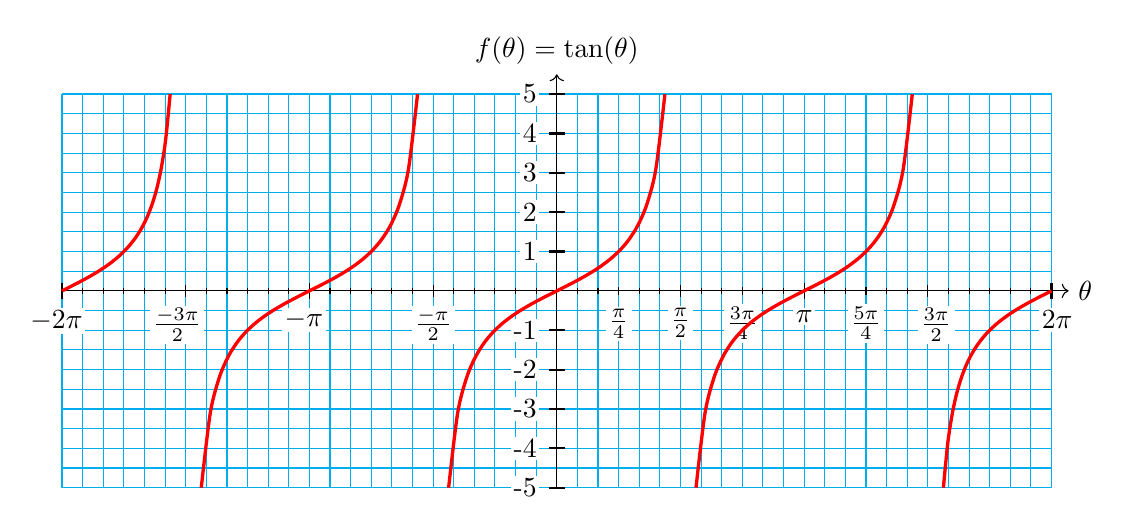
\begin{tikzpicture} [yscale=.5]

\draw[cyan,xstep=pi/12,ystep=0.5]
(-2*pi,-5) grid (2*pi,5);

\draw[->] (-6.3,0) -- (6.5,0) node[right] {$\theta$};
\draw[->] (0,-5) -- (0,5.5) node[above] {$f(\theta)=\tan(\theta)$};

\foreach \x in {-24,-23,...,24}
\draw[black] ($ pi*\x /12*(1,0) +(0,.08) $) --++(0,-.16);
\foreach \y in {-5,-4,...,-1,1,2,...,5}
\draw[black, thick] (.10,\y ) --++(-.2,0) node[anchor=east, xshift=-3, fill=white, inner sep=1pt] {\y};

\draw[black, thick] (-2*pi,.2) --++(0,-.4) node[anchor=north, xshift=-2,yshift=-3, fill=white, inner sep=1pt] {$-2\pi$};
\draw[black, thick] (2*pi,.2) --++(0,-.4) node[anchor=north, xshift=2,yshift=-3, fill=white, inner sep=1pt] {$2\pi$};

\draw[black] (pi,.2) --++(0,-.4) node[anchor=north, yshift=-3, fill=white, inner sep=1pt] {$\pi$};

\draw[black] (pi,.2) --++(0,-.4) node[anchor=north, yshift=-3, fill=white, inner sep=1pt] {$\pi$};
\draw[black] (-pi,.2) --++(0,-.4) node[anchor=north, xshift=-2,yshift=-3, fill=white, inner sep=1pt] {$-\pi$};
\draw[black] (-pi/2,.15) --++(0,-.3) node[anchor=north, yshift=-3, fill=white, inner sep=1pt] {$\frac{-\pi}{2}$};
\draw[black] (pi/2,.15) --++(0,-.3) node[anchor=north, yshift=-3, fill=white, inner sep=1pt] {$\frac{\pi}{2}$};
\draw[black] (3*pi/2,.15) --++(0,-.3) node[anchor=north,xshift=3, yshift=-3, fill=white, inner sep=1pt] {$\frac{3\pi}{2}$};
\draw[black] (-3*pi/2,.15) --++(0,-.3) node[anchor=north,xshift=-3, yshift=-3, fill=white, inner sep=1pt] {$\frac{-3\pi}{2}$};

\draw[black] (pi/4,.11) --++(0,-.22) node[anchor=north, yshift=-4, fill=white, inner sep=1pt] {$\frac{\pi}{4}$};

\draw[black] (3*pi/4,.11) --++(0,-.22) node[anchor=north, yshift=-3, fill=white, inner sep=1pt] {$\frac{3\pi}{4}$};

\draw[black] (5*pi/4,.11) --++(0,-.22) node[anchor=north, yshift=-3, fill=white, inner sep=1pt] {$\frac{5\pi}{4}$};

\foreach \i in {-1, 0, 1}
	\draw[domain={\i*pi-atan(5)*pi/180}:{\i*pi+atan(5)*pi/180}, smooth, variable=\x,red,very thick] plot ({\x},{tan(deg(\x))}) ;

\draw[domain={-2*pi:atan(5)*pi/180-2*pi}, smooth, variable=\x,red,very thick] plot ({\x},{tan(deg(\x))}) ;
\draw[domain={2*pi-atan(5)*pi/180:2*pi}, smooth, variable=\x,red,very thick] plot ({\x},{tan(deg(\x))}) ;

\end{tikzpicture}
\newline


part A: law of sines a circumscribing circle

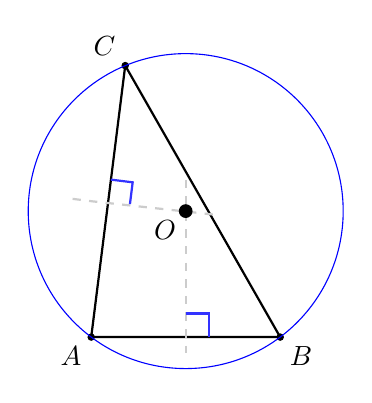
\begin{tikzpicture} [scale=.4]

\coordinate (O) at (0,0);
\coordinate (A) at (-3,-4);
\coordinate (B) at (3,-4);
\coordinate (C) at (-1.92,4.62);

\filldraw (A) circle (.1cm) node[anchor=north east] {$A$};
\filldraw (B) circle (.1cm) node[anchor=north west] {$B$};
\filldraw (C) circle (.1cm) node[anchor=south east] {$C$};

\draw[black,thick] (A)--(B)--(C)--(A);
\draw[gray!40!white, thick, dashed](O)++(0,1) -- (0,-4)--+(0,-.5);
\draw[gray!40!white, thick, dashed](O)++(.862,-.108) -- (-2.96,.31)--++(-.862,.108);
\draw[blue!80!white,thick] (0,-4)++(.75,0)-- ++(0,.75) -- ++(-.75,0);
\draw[blue!80!white,thick] (-2.46,.31) ++(.0864,.6896) -- ++(.6896,-.0864) -- ++(-.0864,-.6896);
\filldraw (O) circle (.2cm) node[anchor=north east] {$O$};

\draw[blue] (O) circle (5);

\end{tikzpicture}
\newline

part B: law of sines a circumscribing circle

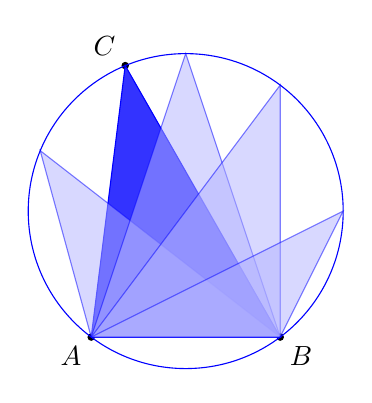
\begin{tikzpicture} [scale=.4]

\coordinate (O) at (0,0);
\coordinate (A) at (-3,-4);
\coordinate (B) at (3,-4);
\coordinate (C) at (-1.92,4.62);
\coordinate (Cp) at (-4.62,1.92);
\coordinate (Cpp) at (0,5);
\coordinate (Cppp) at (3,4);
\coordinate (Cpppp) at (5,0);

\filldraw (O) circle (.1cm) node[anchor=north east] {$O$};
\filldraw (A) circle (.1cm) node[anchor=north east] {$A$};
\filldraw (B) circle (.1cm) node[anchor=north west] {$B$};
\filldraw (C) circle (.1cm) node[anchor=south east] {$C$};

\draw[draw= blue, fill=blue!80!white] (A)--(B)--(C)--(A);
\draw[draw= blue, fill=blue!30!white, opacity=.5] (A)--(B)--(Cp)--(A);
\draw[draw= blue, fill=blue!30!white, opacity=.5] (A)--(B)--(Cpp)--(A);
\draw[draw= blue, fill=blue!30!white, opacity=.5] (A)--(B)--(Cppp)--(A);
\draw[draw= blue, fill=blue!30!white, opacity=.5] (A)--(B)--(Cpppp)--(A);


\draw[blue] (O) circle (5);

\end{tikzpicture}
\newline

Exercise not used?
\begin{tikzpicture}
\coordinate (O) at (0,0);
\coordinate (A) at (0,0);
\coordinate (B) at (0,0);
\coordinate(C) at (0,0);
\coordinate (D) at (0,0);
\filldraw[black] (O) circle (.2pt) node[anchor=south west, xshift=6]{$50\degree$};
\filldraw[black] (A) circle (.2pt) node[anchor=south east]{$x$};
\filldraw[black] (B) circle (.2pt) node[anchor=north east, xshift=-6]{$y$};
\filldraw[black] (C) circle (.2pt) node[anchor=north west]{$z$};
%\draw[black,  thick] (A) -- (B) --( C) -- cycle;
\draw[black] (-2.3,0) --  (2.3,0);
\draw[black] (0.8,1.3) --  (-0.8,-1.3) ;
\end{tikzpicture}
\newline


\end{document}
